% Presentation-only derivative; scripts/build_appendix_compact_tables_20261106.py
\begin{figure}[!htbp]
\centering
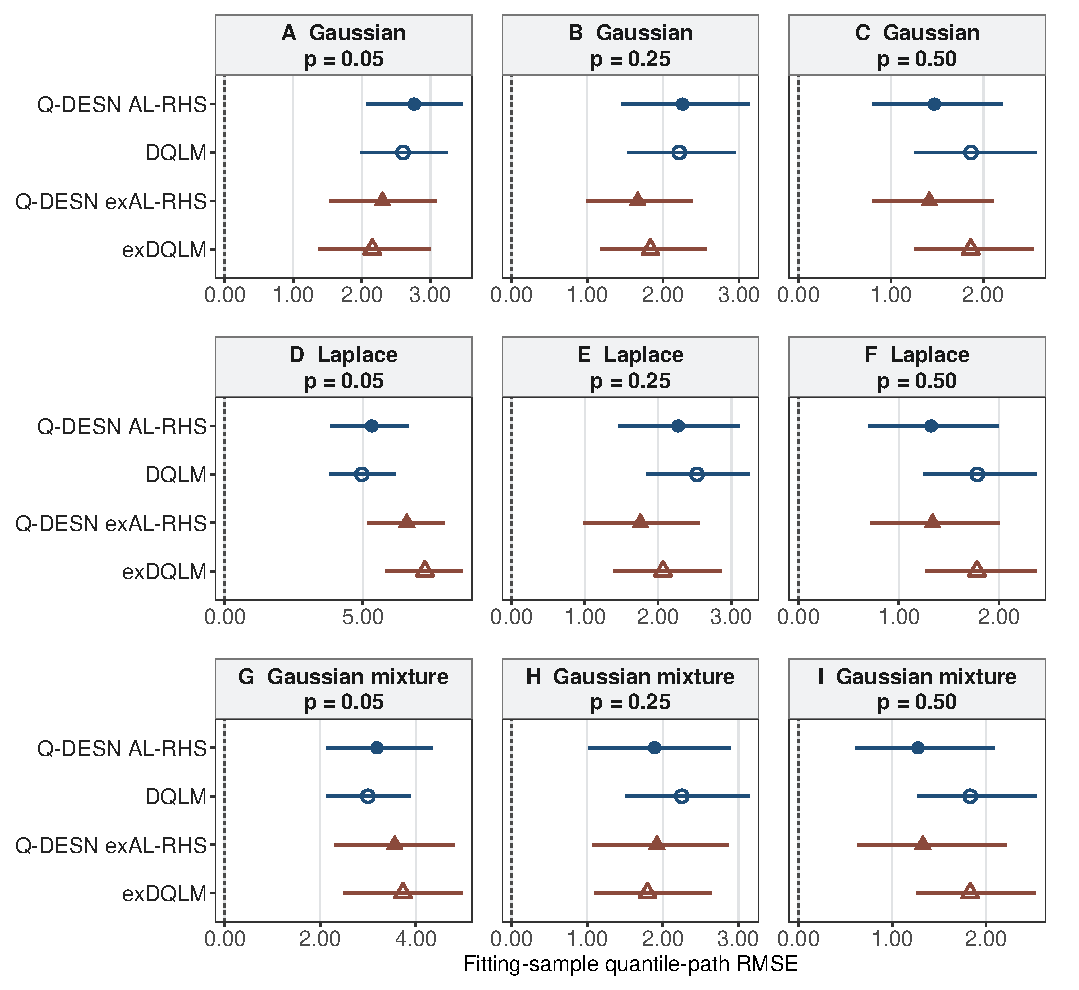
\includegraphics[width=0.98\textwidth]{figures/independent_simulation/qdesn_pro_review_mcmc_fit_rmse.pdf}
\caption{MCMC fitting-sample quantile-path RMSE: means and equal-tailed 95\% intervals conditional on each criterion-specific specification. Colours and symbols follow Figure~\ref{fig:simulation-500obs-mcmc-forecast-mae-intervals}; panels have separate horizontal scales. The dashed line marks exact recovery.}
\figalt{Nine panels compare posterior fitting-sample quantile-path RMSE means
and 95 percent intervals for four models across three observation-error families and
three probability levels. Lower values are better.}
\label{fig:simulation-500obs-mcmc-fit-rmse-intervals}
\end{figure}
